\documentclass[a4paper,12pt]{article}
\usepackage{amsmath, amsthm, amssymb}
\usepackage{tikz} % 添加绘图
\usepackage{tabularx}
\usepackage{enumitem}
\usepackage{fancyref}

\usepackage[top=1in,bottom=1in,left=1in,right=1in]{geometry} % 用于设置页面布局
\usepackage{xeCJK} % 用于使用本地字体
\usepackage[super, square, sort&compress]{natbib} % 处理参考文献
\usepackage{titlesec, titletoc} % 设置章节标题及页眉页脚
%\usepackage{xCJKnumb} % 中英文数字转换
\usepackage{amssymb}
\usepackage{amsmath} % 在公式中用\text{文本}输入中文
\usepackage{diagbox}
\usepackage{multirow} % 表格中使用多行
\usepackage{booktabs} % 表格中使用\toprule等命令
\usepackage{rotating} % 使用sidewaystable环境旋转表格
\usepackage{tabularx}
\usepackage{graphicx} % 处理图片
\usepackage{footnote} % 增强的脚注功能,可添加表格脚注
\usepackage{threeparttable} % 添加真正的表格脚注,示例见README
\usepackage{hyperref} % 添加pdf书签

\usepackage{tikz}
\usetikzlibrary{shapes,arrows,shadows}

% 字体设置
\setmainfont{Times New Roman}
\setsansfont[Scale=MatchLowercase,Mapping=tex-text]{PT Sans}
\setmonofont[Scale=MatchLowercase]{PT Mono}
\setCJKmainfont[ItalicFont={Kaiti SC}, BoldFont={Heiti SC}]{Songti SC}
\setCJKsansfont{Heiti SC}
\setCJKmonofont{Songti SC}
% \setCJKmainfont[BoldFont={FZXiaoBiaoSong-B05S}]{Songti SC}
% \setCJKfamilyfont{kai}[BoldFont=Heiti SC]{Kaiti SC}
% \setCJKfamilyfont{song}[BoldFont=Heiti SC]{Songti SC}
% \setCJKfamilyfont{hei}[BoldFont=Heiti SC]{Heiti SC}
% \setCJKfamilyfont{fsong}[BoldFont=Heiti SC]{Songti SC}
% \newcommand{\kai}[1]{{\CJKfamily{kai}#1}}
% \newcommand{\hei}[1]{{\CJKfamily{hei}#1}}
% \setromanfont[Mapping=tex-text]{TeXGyrePagella}
% \setsansfont[Scale=MatchLowercase,Mapping=tex-text]{TeXGyrePagella}
% \setmonofont[Scale=MatchLowercase]{Courier New}
%%设置常用中文字号,方便调用
\newcommand{\erhao}{\fontsize{22pt}{\baselineskip}\selectfont}
\newcommand{\xiaoerhao}{\fontsize{18pt}{\baselineskip}\selectfont}
\newcommand{\sanhao}{\fontsize{16pt}{\baselineskip}\selectfont}
\newcommand{\xiaosanhao}{\fontsize{15pt}{\baselineskip}\selectfont}
\newcommand{\sihao}{\fontsize{14pt}{\baselineskip}\selectfont}
\newcommand{\xiaosihao}{\fontsize{12pt}{\baselineskip}\selectfont}
\newcommand{\wuhao}{\fontsize{10.5pt}{\baselineskip}\selectfont}
\newcommand{\xiaowuhao}{\fontsize{9pt}{\baselineskip}\selectfont}
\newcommand{\liuhao}{\fontsize{7.5pt}{\baselineskip}\selectfont}

% 章节标题显示方式及页眉页脚设置
% \item xCJKnumb是自己额外安装的包
% \item titleformat命令定义标题的形式
% \item titlespacing定义标题距左、上、下的距离
\titleformat{\section}{\raggedright\large\bfseries}{\thesection}{1em}{}
\titleformat{\subsection}{\raggedright\normalsize\bfseries}{\thesubsection}{1em}{}
\titlespacing{\section}{0pt}{*0}{*2}
\titlespacing{\subsection}{0pt}{*0}{*1}
% 由于默认的2em缩进不够,所以我手动调整了,但是在windows下似乎2.2就差不多了,或者是article中没有这个问题
\setlength{\parindent}{2.2em}

% 设置表格标题前后间距
\setlength{\abovecaptionskip}{0pt}
\setlength{\belowcaptionskip}{0pt}


\renewcommand{\refname}{\bfseries{参~考~文~献}} %将Reference改为参考文献(用于 article)
% \renewcommand{\bibname}{参~考~文~献} %将bibiography改为参考文献(用于 book)
\renewcommand{\baselinestretch}{1.38} %设置行间距
\renewcommand{\figurename}{\small\ttfamily 图}
\renewcommand{\tablename}{\small\ttfamily 表}


\newcommand{\specialcell}[2][c]{%
  \begin{tabular}[#1]{@{}c@{}}#2\end{tabular}}

\newtheorem{proposition}{命题}

\title{在庞加莱圆盘上看加法与乘法}
\author{苑明理}
\date{2017年9月}

\begin{document}

\maketitle{}

\renewcommand\contentsname{目录}
\setcounter{tocdepth}{2}
\tableofcontents

\newpage

\section{预备知识}

\subsection{数字的表示}

我们采用波兰表达式的记法,用两个操作 i 和 d ,以及出发点 0 和 1 ,来表示出不同的数字,其中:

\begin{itemize}
\item i 表示 increase,即加一的操作
\item d 表示 double,即乘二的操作
\end{itemize}

我们作示例如下表

\begin{table}[tbhp]
\centering
\begin{tabularx}{\textwidth}
{|>{\setlength\hsize{0.9\hsize}\setlength\linewidth{\hsize}}X
 |>{\setlength\hsize{0.9\hsize}\setlength\linewidth{\hsize}}X
 |>{\setlength\hsize{0.9\hsize}\setlength\linewidth{\hsize}}X
 |>{\setlength\hsize{0.9\hsize}\setlength\linewidth{\hsize}}X
 |>{\setlength\hsize{0.9\hsize}\setlength\linewidth{\hsize}}X
 |>{\setlength\hsize{0.9\hsize}\setlength\linewidth{\hsize}}X
 |>{\setlength\hsize{0.9\hsize}\setlength\linewidth{\hsize}}X|}
\hline
数字 & 1 &  2 &  3 &  4 &  5 & 6 \\
\hline
不同表示 &
\begin{itemize}[leftmargin=*]\item i0\end{itemize} &
\begin{itemize}[leftmargin=*]\item ii0\item d1\end{itemize} &
\begin{itemize}[leftmargin=*]\item iii0\item id1\end{itemize} &
\begin{itemize}[leftmargin=*]\item iiii0\item iid1\item dii0\item dd1\end{itemize} &
\begin{itemize}[leftmargin=*]\item iiiii0\item iiid1\item idii0\item idd1\end{itemize} &
\begin{itemize}[leftmargin=*]\item iiiii0\item iiiid1\item iidii0\item iidd1\item did1\end{itemize} \\
\hline
最短表示 & i0 & d1 & id1 & dd1 & idd1 & did1 \\
\hline
\end{tabularx}
\caption{六个自然数的表示}
\end{table}

\newpage

\subsection{四阶无限边形镶嵌}

双曲平面上有许多非常有趣的镶嵌结构,这里我们展示一种称为四阶无限边形镶嵌的构造。

\begin{figure}[ht]
\centering
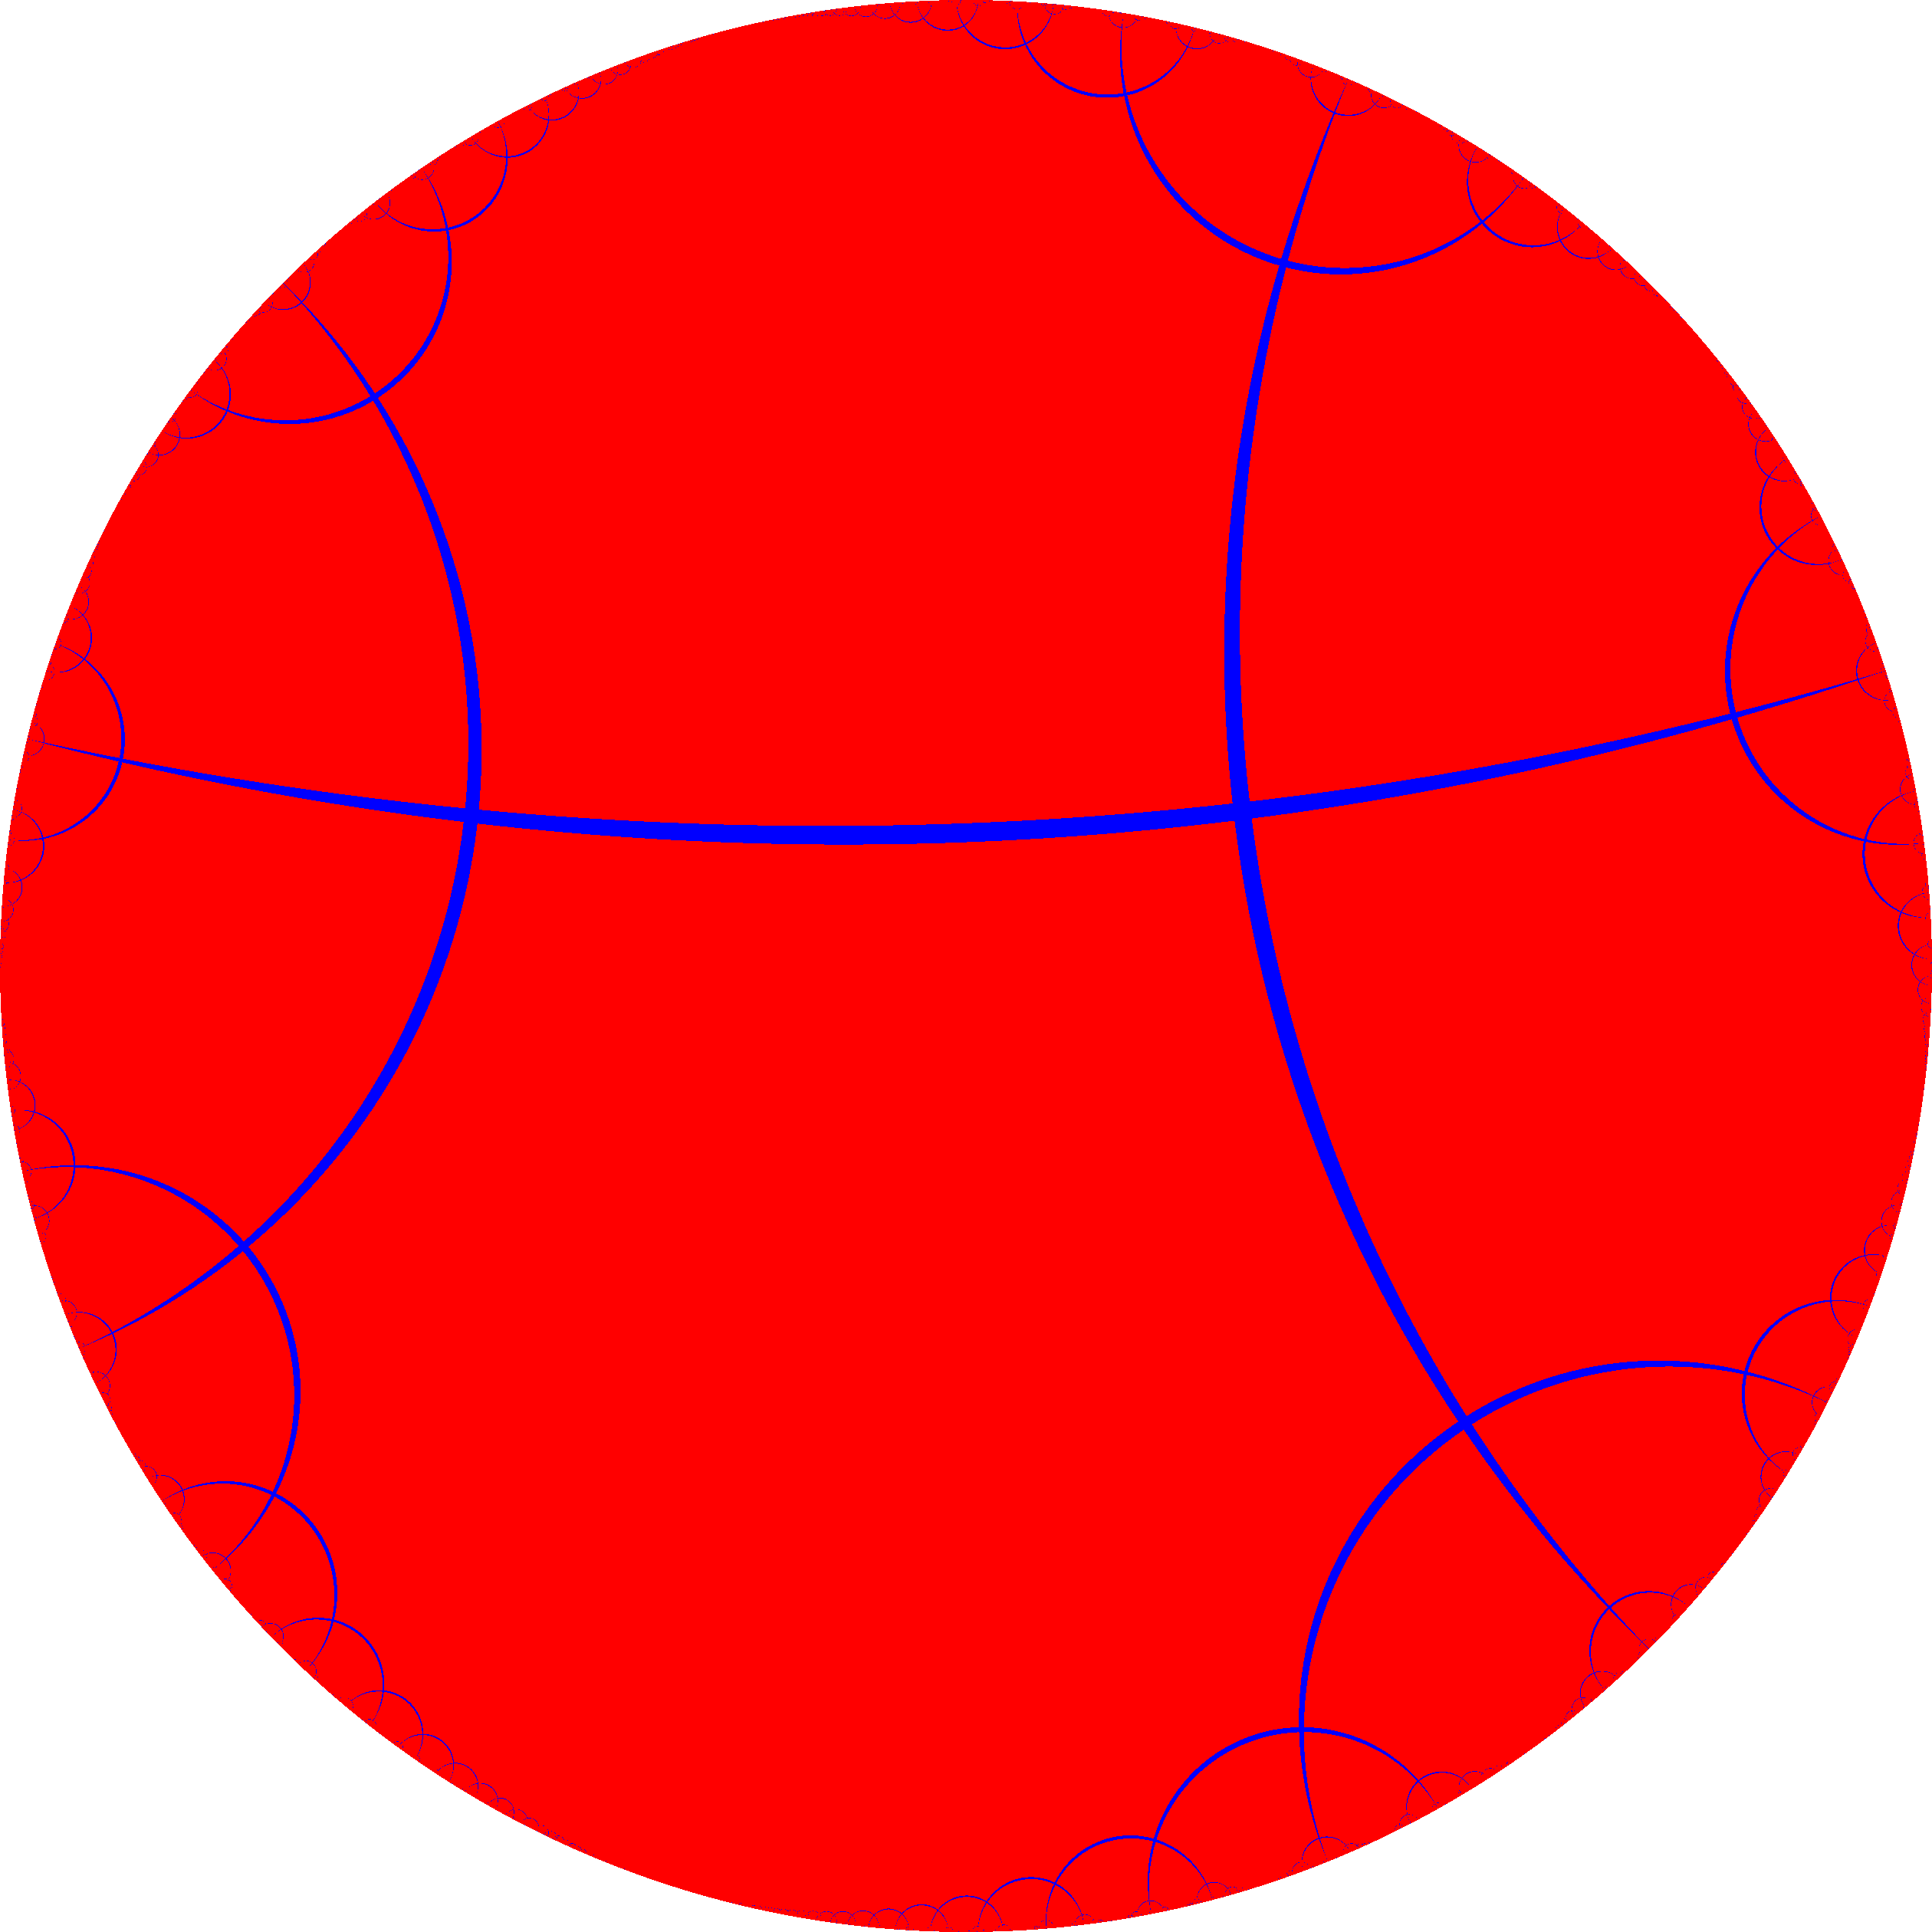
\includegraphics[width=3.5in]{images/H2_tiling_24i-1.png}
\caption{四阶无限边形镶嵌}
\end{figure}

如果注意到双曲平面是一个齐性空间,并且观察到在上述构造里,有些蓝色测地线之间彼此有交点,但这些交点彼此之间没有任何差别;
利用对称性,我们容易理解:

\begin{proposition}
\label{A}
镶嵌结构上的两条测地线如果彼此之间相交,那么它们就是垂直的;否则这两条测地线就是平行的。
\end{proposition}

\begin{proposition}
\label{B}
对于任意一条镶嵌结构上的测地线,镶嵌结构上的其他测地线可以被归类到与之平行或垂直的两组之中。
\end{proposition}

\newpage

\section{操作序列与几何}

\subsection{嵌入到镶嵌结构}

给定镶嵌结构上的一条测地线和一个零点,根据 \ref{B} 的结果,我们称与之平行的所有镶嵌结构上的测地线是加性的,
而与之垂直的所有镶嵌结构上的测地线是乘性的。

接着,我们把操作嵌入进来:赋予加性测地线上两个相邻交点之间的连线的含义为操作 i;赋予乘性测地线上两个相邻交点之间的连线的含义为操作 d。

\begin{proposition}
\label{C}
所有可能的操作序列都被嵌入到镶嵌结构上。
\end{proposition}

\begin{proposition}
\label{D}
从规定的零点开始,所有镶嵌结构上的路径,都是合法的操作序列。
\end{proposition}


\subsection{希尔伯特曲线}

\section{一种新的Surreal数?}

\end{document}
